%\documentclass{beamer}
\documentclass[10pt]{beamer}
\include{mit-beamer-template}
\titleimage{fortrancomic}

\usepackage{amsmath,amssymb,enumerate,calc,color,ifthen,capt-of,booktabs,graphicx,listings,algorithm2e,palatino,amsbsy,bm}

\usefonttheme{serif}

\definecolor{light-gray}{gray}{0.95}
\lstset{basicstyle=\tiny\ttfamily,
        numbers=left,
        backgroundcolor=\color{light-gray},
        frame=shadowbox, 
        rulesepcolor=\color{mitred},
        keywordstyle=\color[rgb]{0,0,1},
        commentstyle=\color[rgb]{0.133,0.545,0.133},
        stringstyle=\color[rgb]{0.627,0.126,0.941}}


\newcommand{\cov}{{$\, \mathbf{C}_{\sigma\sigma} \,$}}
\newcommand{\keff}{$k_{\text{eff}}$ }
\newcommand{\ie}{\textit{i.e. }}
\newcommand{\eg}{\textit{e.g. }}


%---TITLE AND AUTHOR INFORMATION
\title % (optional, use only with long paper titles)
[Criticality Safety]{Criticality Safety}
\author[Roberts]{Jeremy Roberts}
\institute[22.106] % (optional, but mostly needed)
 {}
% - Keep it simple, no one is interested in your street address.
\date
%[CFP 2003] % (optional, should be abbreviation of conference name)
{01/31/2012}


\begin{document}

% TITLE PAGE
\begin{frame}[plain]
  \titlepage
\end{frame}

% TABLE OF CONTENTS
\begin{frame}{Outline}
  \tableofcontents
  % You might wish to add the option [pausesections]
\end{frame}

\begin{frame}{References, etc.}
\begin{enumerate}
 \item R. Knief, {\it Criticality Safety: Theory and Practice}, ANS (1985)
 \item R. Pevey, ``Neutronics'', in {\it Nuclear Engineering Handbook},
       Ed. D. Kok, CRC (2009)
 \item ``A Review of Criticality  Accidents,'' Los Alamos National Laboratory,
       LA-13638 (2000)
 \item Broadhead et al. ``Sensitivity- and Uncertainty-based Criticality 
       Safety Validation Techniques,'' NSE, {\bf 146} (2004)
 \item Various ANSI/ANS Standards, and a bit from 10CFR
\end{enumerate}
\end{frame}

%*******************************************************************************
\section{Overview}

%===============================================================================
\begin{frame}{Nuclear Criticality Safety}

{\bf American National Standard ANSI/ANS-8.1}:
\vfill
{\it criticality safety}: protection against the consequences of a criticality 
safety accident, preferably by prevention of the accident
\vfill
{\it criticality accident}: the release of energy as a 
result of accidental production of a self-sustaining or
divergent neutron chain reaction
\vfill 
ANSI/ANS-8.1 
\begin{itemize}
 \item provides general guidance for  nuclear criticality safety 
       applied to fissionable materials \textit{outside} of reactors
 \item produced and updated by working groups within ANS (with significant
       association to NCSD of ANS)
\end{itemize}

\end{frame}

%===============================================================================
\begin{frame}{Relevant Standards}

\begin{table}[ht]
    \caption{Several ANSI/ANS Standards Applicable to Criticality Safety.}
    \begin{center} 
    \begin{tabular*}{1.00\textwidth}{@{\extracolsep{\fill}} p{3cm}p{0.9\textwidth-3cm} } 
      \toprule 
        Number-Revised    &  Title \\
      \midrule
       8.1-1998                  &  Nuclear Criticality Safety in Operations 
                                    with Fissionable Materials Outside 
                                    Reactors \\
       8.3-1997                  &  Criticality Accident Alarm System \\
       8.5-1996                  &  Guide for Nuclear Criticality Safety in 
                                    the Storage of Fissile Materials \\
       8.17-2004                 &  Criticality Safety Criteria for the 
                                    Handling, Storage, and Transportation 
                                    of LWR Fuel Outside Reactors \\
       8.24-2007                 &  Validation of Neutron Transport 
                                    Methods for Nuclear Criticality Safety 
                                    Calculations \\
       8.27-2008                 &  Burnup Credit for LWR Fuel \\
      \bottomrule 
    \end{tabular*} 
    \end{center} 
    \label{tbl:ansstandard}
\end{table}

\end{frame}

%===============================================================================
\begin{frame}{Other Oversight}

{\bf Nuclear Regulatory Commision}:
\vfill
{\it NUREG}: documents produced by NRC, contractors, or via international
agreements
\vfill
{\it 10CFR}: mostly parts 0, 1, 2, 20, and several between 50 and 75
\vfill
\textcolor{mitred}{Homework}: go look up one or more relevant NUREG documents or parts 10CFR and
explain the relevance.

\end{frame}

%===============================================================================
\begin{frame}{Historical Footnote}

Nuclear criticality safety is {\it about} as old as other nuclear engineering
disciplines.  Feynman might have started it all in Oak Ridge; he delivered
Oppenheimer's message, stating
\vfill
\textcolor{mitred}{``Los Alamos cannot accept the responsibility
for the safety of the Oak Ridge plant unless they are full informed as
to how it works.''}
\vfill
and went on to explain
\vfill
\textcolor{mitred}{``\ldots all about neutrons, how they worked, da da, ta ta ta,
there are too many neutrons together, you've got to keep the material
apart, cadmium absorbs \ldots''}
\vfill
(from {\it Surely You're Joking, Mr. Feynman})

\end{frame}


%*******************************************************************************
\section{Physical Concerns}

%===============================================================================
\begin{frame}{What Parameters Matter?}
\pause
\begin{enumerate}
 \item mass
 \item concentration
 \item enrichment
 \item volume
 \item absorption
 \item moderation
 \item reflection
 \item interaction
\end{enumerate}
\vfill Easy to remember: {\bf MAGICMERV}.
\end{frame}

%===============================================================================
\begin{frame}{Simple Example}
  \begin{figure}
    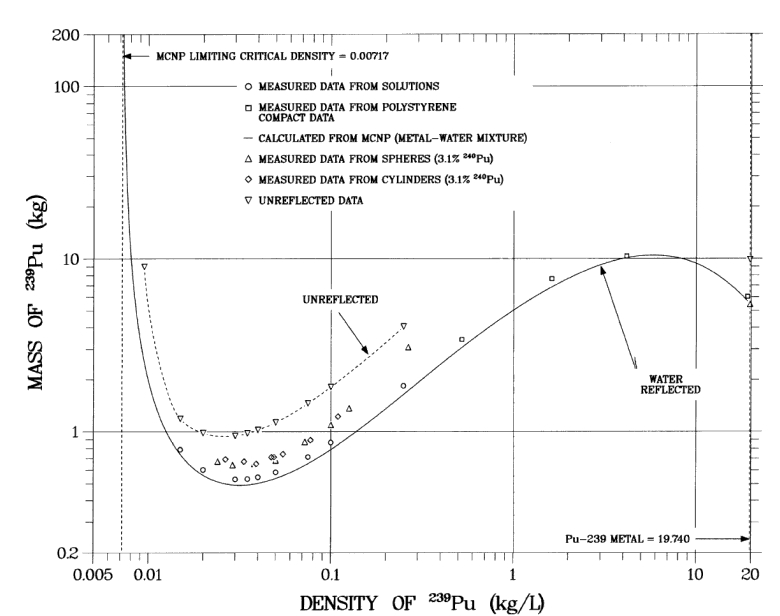
\includegraphics[keepaspectratio, width = 3.2 in]{images/pu_critical_mass}
    \caption{Pu-239 solution critical mass. (Borrowed from Martin, J. {
             {\it Physics for Radiation Protection: A Handbook}}, Wiley (2016).}
  \end{figure}
\end{frame}


%*******************************************************************************
\section{Accidents}

%===============================================================================
\begin{frame}[fragile]{A Simple Model}

An accident is an {\it excursion}, an uncontrolled reaction; {\it we can
model this}.
\vfill
Time to remember your reactor kinetics!
\end{frame}

%===============================================================================
\begin{frame}[fragile]{A Simple Model - Definition}

Reactivity:
\begin{equation}
 \rho = \frac{k-1}{k} 
\end{equation}
Time-dependent population:
\begin{equation}
  n(t) =  n_o e^{\frac{\rho-\beta}{l}t}
\end{equation}
where
\begin{itemize}
 \item $\beta$ is the delayed neutron fraction ($\approx 0.007$)
 \item $l$ is the neutron lifetime ($\approx 1\cdot 10^{-5}$ s)
\end{itemize}

\end{frame}

%===============================================================================
\begin{frame}[fragile]{A Simple Model - Application}

Suppose:
\begin{itemize}
 \item $n_0 = 1$
 \item $l = 10^{-5}$ s
 \item $\rho-\beta = 0.002$
 \item $\Delta t = 0.200$ s
 \item 1 rem corresponds to a fluence of  $27\cdot 10^6$  n/cm$^2$
\end{itemize}
\vfill
\textcolor{mitred}{Question}: what's a dose to a worker a half-meter away?
  Is it bad? How bad?

\end{frame}

%===============================================================================
\begin{frame}[fragile]{The Plutonium Sphere}

  \begin{figure}
    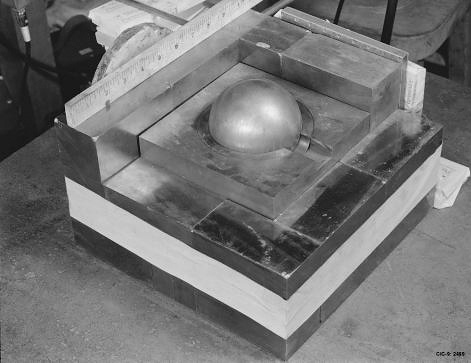
\includegraphics[keepaspectratio, width = 3.2 in]{images/pu_sphere}
    \caption{From the LANL Review.}
  \end{figure}

\end{frame}

%===============================================================================
\begin{frame}{The Plutonium Sphere}

Summary:
\begin{itemize}
 \item August 21, 1945
 \item 6.2 kg plutonium sphere coated with nickel
 \item tungsten carbide brick (reflector)
 \item while placing blocks, experimenter dropped one onto sphere
 \item supercritical excursion yielded $10^{16}$ fissions and a (fatal)
       dose of 510 rem
\end{itemize}
\vfill
\textcolor{mitred}{How does this compare to the simple example?}

\end{frame}

%===============================================================================
\begin{frame}{Tickling the Dragon's Tail}

  \begin{figure}
    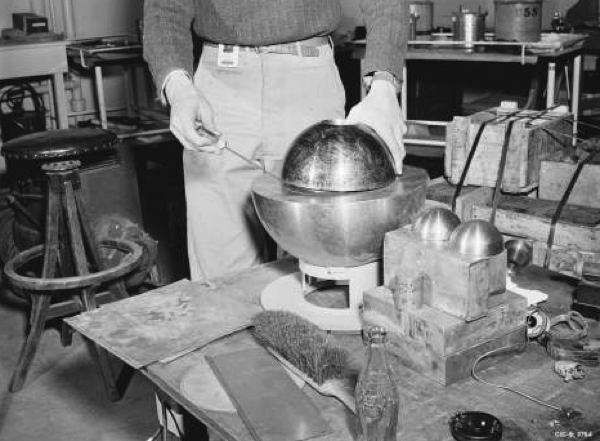
\includegraphics[keepaspectratio, width = 3.2 in]{images/pu_sphere_2}
    \caption{From the LANL Review.  Experimenter died, and significant dose
             to several observers.  Same sphere as the last one, just a half 
             year later!}
  \end{figure}

\end{frame}

%===============================================================================
\begin{frame}{Process Accident at Y-12}

Summary:
\begin{itemize}
 \item June, 16 1958
 \item Y-12 produces parts from HEU (in Oak Ridge, TN)
 \item accident occurred in area for HEU recovery
 \item storage tanks to be cleaned and leak-tested with water
 \item U-solution built up below tanks (and into one) via leak from process 
       stream
 \item subsequent leak-test resulted in accumulation in 55 g drum; a worker 
       described yellow-brown fumes followed by blue light...
 \item no fatalities, but eight workers with significant doses
\end{itemize}

\end{frame}

%===============================================================================
\begin{frame}{Tokai-mura, Japan}

{\it Criticality accidents are not just a relic of the past!}
\vfill
Summary:
\begin{itemize}
 \item September, 29 1999 (and into October, 1)
 \item occurred at uranium conversion facility
 \item workers placed 16.6 kg of 18.8\%
       enriched uranium into a tank designed to contain no more than
       2.4 kg of uranium at such high enrichments
 \item accident was the first of its kind in Japan, and the first 
       resulting in casualties
 \item criticality was maintained intermittently for roughly 20 hours before 
       effective action was taken
\end{itemize}

\end{frame}

%*******************************************************************************
\section{Computational Aspects}

%===============================================================================
\begin{frame}{Computational Aspects: Overview}

Goal: understand how computational tools are used and validated within
      criticality safety analysis; this includes
\begin{enumerate}
 \item subcritical limits
 \item criticality safety analysis validation
 \item computational bias determination via traditional techniques (e.g.
       trending analysis)
 \item new techniques based on S/U analysis and their application to 
       a relevant current problem
\end{enumerate}

\end{frame}

\begin{frame}{Subcritical Limit}

{\bf ANSI/ANS 8.1}: ``the 
limiting value assigned to a controlled parameter that results in a subcritical 
system under specified conditions. The parameter limit allows for 
uncertainties in the calculations and experimental data used in the derivation 
but not for contingencies.''
\vfill
These are \textit{absolute maxima}: no contingincies! An administrative
margin is needed.
\end{frame}

\begin{frame}[fragile]{Control Parameters}
\begin{table}[ht]
    \caption{Example single parameters and subcritical limits.}
    \begin{center} 
    \begin{tabular*}{0.99\textwidth}{@{\extracolsep{\fill}} ll } 
      \toprule 
        parameter &  example limit \\
      \midrule
       fissile mass                    &  0.78 kg  ${}^{235}$U in UO$_2$NO$_3$ \\
       dimension (width, volume, etc.) &  6.2   L  ${}^{235}$U in UO$_2$NO$_3$ \\
       concentration                   &  11.6 g/L ${}^{235}$U in UO$_2$NO$_3$ \\
       enrichment                      &  5\%      ${}^{235}$U in UO$_2$       \\
       fissile mass                    &  20.1 kg  ${}^{235}$U in UO$_2$ 
                                          ($\rho \leq 18.81$ g/cc) \\
      \bottomrule 
    \end{tabular*} 
    \end{center} 
    \label{tbl:controlparams}
\end{table}
\vfill
Multiple parameters possible, but stricter administrative margins required.

\end{frame}


\begin{frame}{Criticality Safety Analysis Validation}

Single parameter (and even multiple parameter) limits are useful but
limited.  
\vfill
Two questions arise:
\begin{enumerate}
 \item how does one actually establish these limits?
 \item how does one ensure subcriticality in complex systems?
\end{enumerate}

\end{frame}

\begin{frame}{Areas of Applicablility}

ANSI/ANS 8.1 requires methods be valid an within the ``areas of 
applicability'' for a given application.  It defines:
\vfill
{\it area of applicability}:  limiting 
ranges of material compositions, geometric arrangements, neutron energy 
spectra, and other relevant parameters \ldots within which the bias of the 
computational method is established
\vfill
{\it computational bias}:  systematic 
discrepancy between and experimental data and calculated results (with
associated uncertainties)

\end{frame}

\begin{frame}{Establishing Subcriticality}

ANSI/ANS 8.17 requires:

\begin{equation}
 k_a + \Delta k_a \leq k_c - \Delta k_c \, ,
\end{equation}
or
\begin{equation}
 k_a \leq k_c  - \Delta k_a - \Delta k_c \, .
\end{equation}
and for more conservatism
\begin{equation}
 k_a \leq k_c - \Delta k_a - \Delta k_c - \Delta k_m \, .
\end{equation}
Here, $k_a$ is the {\it most conservative} estimate for the application $k$,
and $k_c$ is the {\it least conservative} estimate $k$ from experiment.  
The $\Delta k$'s represent uncertainties and an administrative margin 
(typically 5\%).

\end{frame}

\begin{frame}{Upper Subcritical Limit}

Rewrite the previous equation as
\begin{equation}
 k_a + \Delta k_a + \Delta k_m - \beta + \Delta \beta \leq 1 \, ,
\label{eq:kallow}
\end{equation}
where the bias is
\begin{equation}
 \beta = k_c - 1 \, ,
\end{equation}
and its uncertainty is
\begin{equation}
 \Delta \beta = \Delta k_c \, .
\end{equation}
\vfill
The {\it upper subcritical limit} (USL) is defined
\begin{equation}
 USL = 1 - \Delta k_m + \beta - \Delta \beta  .
\end{equation}
Note that $k_a + \Delta k_a \leq USL$, so the USL \textcolor{mitred}
{is the maximum value an 
application \keff (plus any uncertainties) may have for which the 
application can, with a high degree of confidence, be considered 
subcritical.}

\end{frame}

\begin{frame}{Traditional Bias Determination}

Traditional approach is {\it trending analysis}: 
\begin{enumerate}
 \item A set of of experiments ``similar'' to an application are selected
 \item Experiments and experimental models are correlated for a given
       parameter 
 \item A bias is determined as a function of the parameter and applied
       via interpolation (or extrapolation with additional margin) to 
       the application system 
\end{enumerate}
Common trending variables include
\begin{itemize}
 \item enrichment
 \item average energy causing fission (EAF)
 \item energy of average lethargy causing fission (EALF)
 \item H/X 
\end{itemize}

\end{frame}

\begin{frame}{One Approach: USL$_1$}

Basic idea (details in uploaded notes):
\begin{itemize}
 \item Find $k_c(p)$ as a function of parameter $p$; $\beta(p) = 1 - k_c(p)$. 
       Note, $\beta < 0$ is to be avoided; current practice sets 
       $\beta > 0$ to zero.
 \item Compute a lower confidence band $w(p)$ statistically (based on a 
       student-t distribution); any negative
       $\beta$ is no worse than $1 - w(p)$.
 \item For convenience, define $W$ as the most limiting value of $w$ at the
       limits of the range of $p$; $W$ typically computed at a 95\% 
       confidence level
\end{itemize}

\end{frame}

\begin{frame}{S/U Techniques - 1}

Motivation: selection of parameters and experiments subject to expert
judgment, and new designs may be outside area of applicability of 
current data.
\vfill
Possible solution: DOE's Nuclear Criticality Safety Program aimed to
develop \textcolor{mitred}{a rigorous physics-based approach for the 
determination of system similarity} based on S/U analysis
\pause
\vfill
Relative sensitivity of \keff to a nuclide-reaction $x$:
\begin{equation}
 S_{k,\sigma_x} = \frac{\sigma_x}{k}\frac{\partial k}{\partial \sigma_x} 
\end{equation}
In vector form, $\mathbf{S}$ useful for comparing two systems
both {\it qualitatively} and {\it quantitatively}.
\end{frame}

\begin{frame}{S/U Techniques - 2}
Let a set of group-wise, nuclide-reaction cross-sections be denoted 
\begin{equation}
 \bm{\sigma} \equiv \sigma_i, \; \; n = 1,\;2,\ldots,N
\end{equation}
with relative covariance matrix
\begin{equation}
 \mathbf{C_{\sigma \sigma}} \equiv 
   \Bigg[\frac{\mathrm{COV}(\sigma_i,\sigma_j)} {\sigma_i \sigma_j} \Bigg ] \, .
\end{equation}
The uncertainty in \keff is therefore
\begin{equation}
\frac{\delta k}{k} = \sqrt{ \mathbf{S}_k \mathbf{C_{\sigma \sigma}} 
                     \mathbf{S}_k^T } \, ,
\end{equation}

\end{frame}

\begin{frame}{S/U Techniques - 3}
For several systems $I$, $\mathbf{\bar{S}}_k$ is an $N \times I$ matrix,
and
\begin{equation}
 \mathbf{C}_{kk} =  \mathbf{\bar{S}}_k \mathbf{C_{\sigma \sigma}} 
                    \mathbf{\bar{S}}_k^T  
\end{equation}
is the associated $I\times I$ covariance matrix with entries $\alpha_{ij}$.
\vfill
The correlation coefficient between system $i$ and $j$ is defined
\begin{equation}
 c_{k} =  \frac{\alpha^2_{ij}}{\alpha_i \alpha_j}  \, ,
\end{equation}
and ranges from -1 to 1.  Like enrichment or EALF, $c_k$ can be
used in trending analyses.
\end{frame}

%===============================================================================
\begin{frame}[fragile]{Example Trending Analysis - 1}
  \begin{figure}
    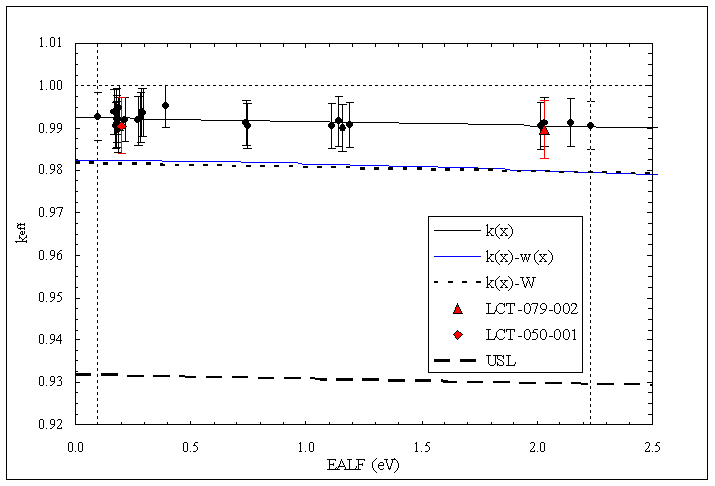
\includegraphics[keepaspectratio, width = 3.2 in]{images/trend_ealf}
    \caption{All systems are LEU experiments in IHECSBE.  Two were selected
             as sample applications.  Here, EALF is used to trend.}
  \end{figure}
\end{frame}

\begin{frame}[fragile]{Example Trending Analysis - 2}
  \begin{figure}
    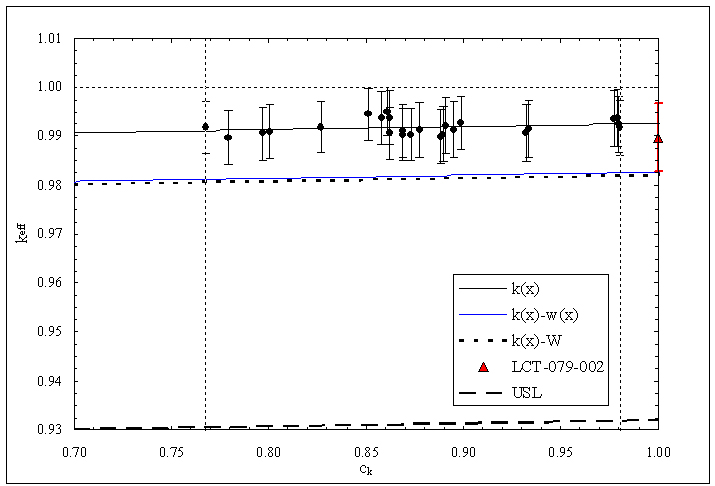
\includegraphics[keepaspectratio, width = 3.2 in]{images/trend_ck1}
    \caption{Here, $c_k$ specific to one of the sample applications is used.}
  \end{figure}
\end{frame}

\begin{frame}[fragile]{Example Trending Analysis - 3}
\begin{table}[hp]
 \caption{Observed and predicted biases ($\beta_{\mathrm{ob}}$ and 
         $\beta$), $\Delta \beta$, all in percent, and USL using 
         each trending technique.}
 \begin{center} 
 \begin{tabular*}{0.98\textwidth}{@{\extracolsep{\fill}} c|cccc|cccc } 
  \toprule
              & \multicolumn{4}{c}{LCT-079-002}          & \multicolumn{4}{c}{LCT-050-001} \\
   \midrule 
             & $\beta_{\mathrm{ob}}$ & $\beta$ & $\Delta \beta$  & USL & $\beta_{\mathrm{ob}}$& $\beta$  & $\Delta \beta$ & USL \\ 
   \midrule
       EALF  &  -1.08  &  -0.95  &  1.08  &  0.9298  &  -0.94  &  -0.77  &  1.08  &  0.9316 \\
    Enrich.  &  -1.08  &  -0.84  &  1.02  &  0.9314  &  -0.94  &  -0.85  &  1.02  &  0.9313 \\
      $c_k$  &  -1.08  &  -0.74  &  1.16  &  0.9306  &  -0.94  &  -0.71  &  1.07  &  0.9322 \\
  \bottomrule 
 \end{tabular*} 
 \end{center} 
 \label{tbl:trendbias}  
\end{table} 
\vfill
Something to note:  all the biases are small and far outweighed by the 5\% adminstrative margin!
\end{frame}

\section{Case Study: Burnup Credit}

\begin{frame}{Burnup Credit}
Burnup Credit: {\it taking into account the reduction in reactivity due to burnup}
\vfill
Why do we care?  {\it Economics.}
  \begin{figure}
    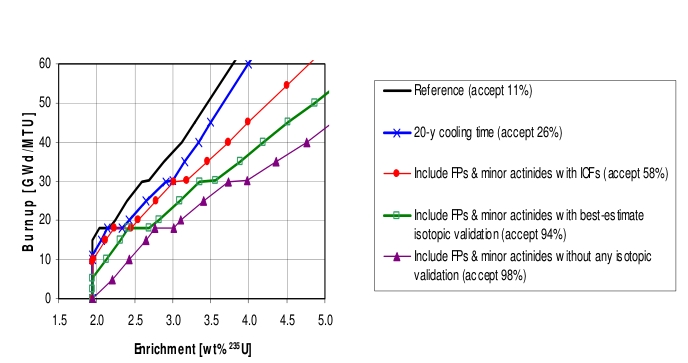
\includegraphics[keepaspectratio, width = 3.5 in]{images/loading_curve}
  \end{figure}
\end{frame}

\begin{frame}{Burnup Credit}
Summary of recent work:
\begin{itemize}
 \item Use S/U tools to extract {\it partial} biases for specific nuclides
 \item GLLSM for data adjustment
 \item Replacement experiments and reactivity differences
 \item Maybe? informed experiment design
\end{itemize}
\vfill
Methods are promising {\it but sensitive to experiment correlation} and
{\it very sensitive to data covariance}; our knowledge of both is dismal!
\end{frame}

\end{document}
